% Compact PGFPlots panel for sampled qldpc_43_4_5_cluster_variant40_cap7 BSC correction-class derivative.
% Requires \usepackage{pgfplots} and \pgfplotsset{compat=1.18}.
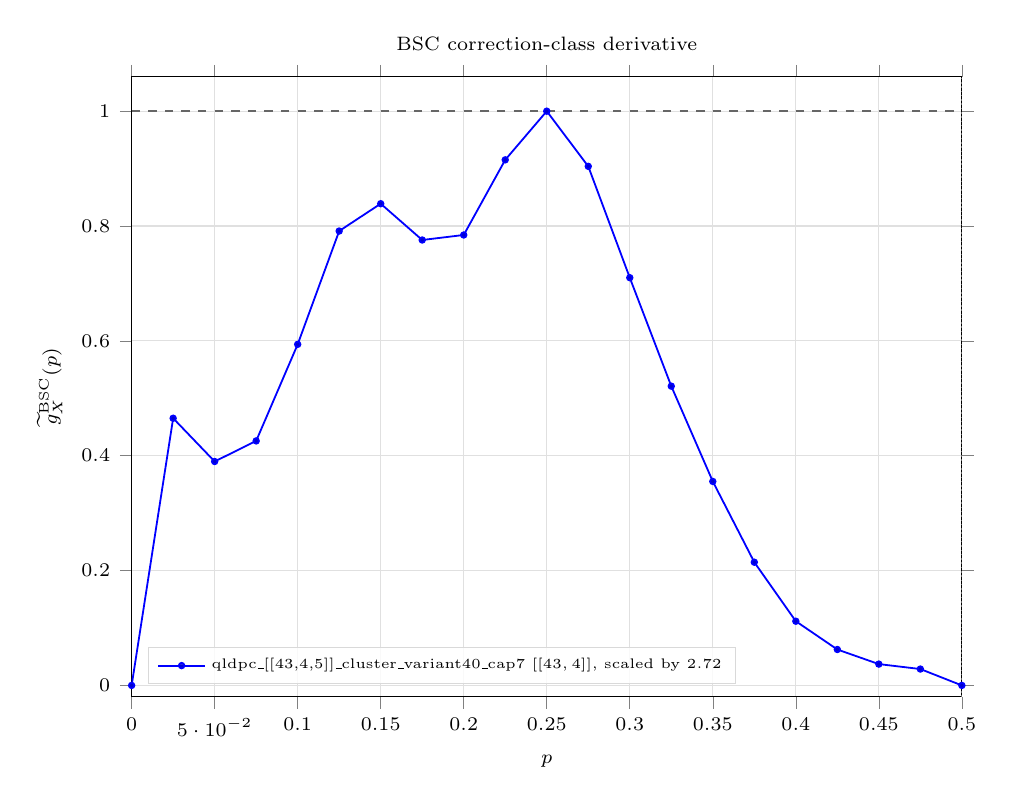
\begin{tikzpicture}
\begin{axis}[
  name=scaledBSCGEXITQldpc4345ClusterVariant40Cap7Axis,
  width=\linewidth,
  height=0.78\linewidth,
  title={BSC correction-class derivative},
  title style={font=\scriptsize},
  xlabel={$p$},
  ylabel={$\widetilde g_X^{\rm BSC}(p)$},
  xmin=0, xmax=0.5,
  ymin=-0.02, ymax=1.06,
  grid=both,
  major grid style={black!12},
  minor grid style={black!6},
  tick align=outside,
  tick label style={font=\scriptsize},
  label style={font=\scriptsize},
  legend cell align={left},
  legend style={draw=black!15, fill=white, fill opacity=0.82, text opacity=1, at={(0.02,0.02)}, anchor=south west, font=\tiny},
]
\addplot[black!60, densely dotted, line width=0.55pt, forget plot] coordinates {(0.5,-0.02) (0.5,1.06)};
\addplot[black!60, dashed, line width=0.55pt, forget plot] coordinates {(0,1) (0.5,1)};
\addplot+[color=blue, mark=*, mark size=1.0pt, line width=0.65pt]
coordinates {(0,0) (0.025,0.465296660822) (0.05,0.389943445139) (0.075,0.425786395754) (0.1,0.593980835938) (0.125,0.791317627933) (0.15,0.838883387872) (0.175,0.775669768751) (0.2,0.78439934876) (0.225,0.915274024753) (0.25,1) (0.275,0.903938831406) (0.3,0.710044983946) (0.325,0.521127184214) (0.35,0.355217522338) (0.375,0.214555049176) (0.4,0.11181112707) (0.425,0.062561404648) (0.45,0.037130504932) (0.475,0.0285297628919) (0.5,0)};
\addlegendentry{qldpc\_[[43,4,5]]\_cluster\_variant40\_cap7 $[[43,4]]$, scaled by $2.72$}
\end{axis}
\end{tikzpicture}
